\chapter{Mixed models (a.k.a. Hierarchical Linear Models or HLM)}\citep{hlm}

\section{Fixed and random effects}

Hierarchical linear models, also known as multilevel level models, are often called mixed models because they include estimates of both fixed and random effects. To understand what this means, it is useful to recall what a fixed effect is, what a random effect is, and under what circumstances do statistical problems require the estimation of both.

Multilevel, mixed, hierarchical, models are a tool for analyzing data where there is a hierarchical structure in which observations are nested within a system of clusters. This can be fish in ponds, students in schools, or more complicated systems where time is nested within individuals who are nested within neighborhoods.

Analysis of such data should never be done using the methods we learn for simple random samples. This includes independent samples t-tests, ordinary least squares regression, and so on. The reason for this is that the formulas for standard errors based on the simple random sample methods assume that all the observations are independently observed. In clustered data, they are not. Thus, the sampling errors assume we have more information than we actually do, because units within clusters tend to be correlated (even a little bit). This leads to smaller standard errors by mistake, leading to significant results that may be by mistake.

Multilevel models that estimate fixed and random effects offer a method to analyze hierarchical data in such a way that it produces the correct standard errors for hypothesis tests. They also produce estimates of fixed effects from a sample of groups that can be generalized to the population of groups. Examples would be treatment effects of an intervention in schools, or other non-causal associations such as age, race, or gender effects.

A lot of data we deal with in the social sciences is clustered, but not all of it should be used with multilevel modeling. The trick to understanding when it is a good idea is to think about the following question: Do you want to generalize beyond your observed groups?

For example, you may have all the census tracts in the United States in your data, which is not a sample of clusters. Thus, one argument would be to not use random effects, but instead employ other methods depending on whether you have tract-level covariates. If you don't have tract level covariates you are interested in modeling, an econometric fixed effect model may be in order, which effectively removes any tract level variance from your model. If you do have tract-level covariates, then perhaps it is appropriate to employ cluster robust standard errors.

However, you may want to generalize to a super-population of tracts, or areas beyond the United States.  Then, your data set may be considered a sample of tracts, and modeling random effects may be appropriate.

In another situation, you may have a set of groups in a study, but you only care about whether your intervention works for that set. This is another case in which your set of clusters may not be considered random, and thus the need to mixed effects model is limited.

Another case in which you do not need to use multilevel models is when you have a complex probability sample, from say, a big national survey that used a cluster sample.  This is common, at NORC we often first sample geographic clusters, then sample areas within those clusters, then people in those areas. This is a hierarchical model, but the research questions may have nothing to do with those geographic areas. If that's the case, there is a whole literature on using probability weights to estimate descriptive and correlation based statistics with appropriate standard errors.

Towards the turn of the century, it seemed that everyone was using multilevel models, and in many situations where it was not required or even appropriate. However, if you have a sample of groups, and/or you want to generalize to some population of groups, and you want the correct standard errors, and/or, are interested in estimating the variance components, then multilevel models will be helpful.


\section{Data}

Let's organize how we will talk about our data. First, for convenience, let's assume a balanced dataset where there are the same number of observations per group. Here, $j$ equals 1, 2, to $m$ groups, with each group having 1, 2, up to $n$ units. Thus, the variable $y_{ij}$ is the $i$th observation from group $j$, and the total number of observations is $N$ equals $m \times n$

\[
y_{ij}
\]
Groups or clusters:
\[
j = \left\{1,2,\dots,m\right\}
\]
Units:
\[
i = \left\{1,2,\dots,n\right\}
\]
Total:
\[
N = m\times n
\]

Suppose we performed an experiment with two treatment conditions, say, Treatment and Control. The linear model of the outcomes observed for each individual $i$ in treatment group $j$ would be the outcome $y_{ij}$ as a function of an overall mean, $\mu$, plus a fixed treatment effect, $\alpha_j$, plus a residual $e_{ij}$

\begin{equation}\label{genlinmod}
  y_{ij} = \mu + \alpha_j+e_{ij}
\end{equation}

\[
\underbrace{y_{ij}}_{\text{outcome}} = \underbrace{\mu}_{\text{overall mean}} + \underbrace{\alpha_j}_{\text{treatment effect}}+\underbrace{e_{ij}}_{\text{residual}}
\]

We will use Greek letters to refer to fixed effects. We also add the constraint that the group effects sum to zero.
\[
\sum_j^m \alpha_j = 0
\]

It is important to understand why we call these fixed effects. The idea is that we are estimating the effect from only a fixed number of treatment conditions. We don't imagine that there are other treatments conditions we created, only a treatment group and a control group. Hence, because there are only a fixed number of possible groups, their effects are fixed effects.

Since the treatment effects are fixed, they do not come from a probability distribution, and so we do not think of a variance of treatment effects. However, we generally think of the residual has coming from a normal random distribution with a mean of zero and a homogenous variance, $\sigma^2_w$, with the w denoting that this is the within-group variance

\begin{equation}
  e_{ij} \sim N\left(0,\sigma^2_w\right)
\end{equation}

So, analyses with fixed effects are really only dealing with one component of variance, the within-group variance. Thus, the variance of the outcome, net of treatment group, is the within group variance alone

\[
\mbox{var}\left(y_{ij}|\alpha_j\right) = \sigma_w^2
\]

Statistical analysis with fixed effects is generally carried out with a t-test for two groups or ANOVA for two or more groups. As you may recall from introductory statistics classes, the ANOVA procedure estimates an F-statistic that is the ratio of the mean-square-between, or $MSB$, groups and the mean-square-within-groups, or $MSW$

\[
F = \frac{MSB}{MSW}
\]

The expected value of the MSB in a fixed effects analysis, where we suspect the alternative hypothesis to be true, is the within-group variance plus a fraction of the group size, n, times the sum of the squared treatment effects  to the number of groups minus one

\[
E[MSB] = \sigma_w^2 + \frac{n\sum_{j=1}^m\alpha_j^2}{m-1}
\]

Which is estimated by the MSB we all learned in our early statistics courses. The expected mean-square-within is simply the within group variance, or the variance of the residuals

\[
E[MSW] = \sigma_w^2
\]

The expected F-test is then a ratio of these values, which under the null hypothesis we expect the result to be a ratio of 1

\[
E[F_{null}] = \frac{\sigma_w^2}{\sigma_w^2}
\]

and under the alternative hypothesis the expected value is a ratio greater than 1 because we add the treatment effects to the numerator

\[
E[F_{alternative}] = \frac{\sigma_w^2+\frac{n\sum_{j=1}^J\alpha_j^2}{J-1}}{\sigma_w^2}
\]

To summarize, fixed effects models deal with outcomes that are grouped by variables that contain all the clusters of interest. These are usually analytic variables such as treatment conditions, gender, race, etc. Next, we move to analysis situations in which the grouping variable does not contain all the groups of interest, but instead a sample of them.

Next, we consider random effects. Unlike fixed effects, where we have all the groups of interest such as treatment and control conditions, a random effects model considers inference to all possible groups from a sample of groups. For example, suppose we want to generalize our results of an analysis of students in schools to all schools, but by employing only a sample of schools. One research question could be, analogous to treatment effects, whether all schools have the same average outcome.

\begin{figure}
  \centering
  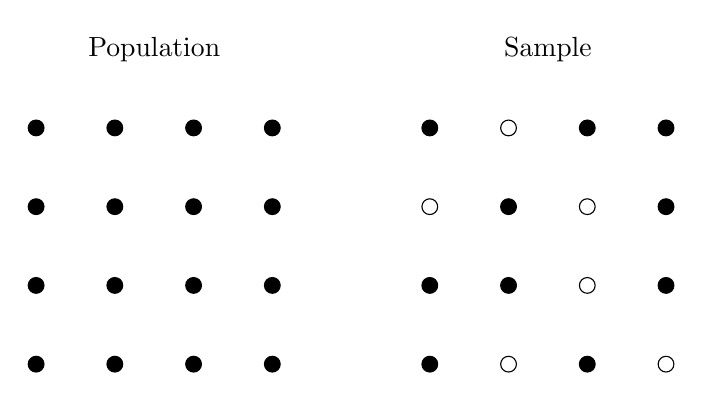
\begin{tikzpicture}
\node at (2.5,6) {Population};
\draw [fill] (1,2) circle [radius=0.1];
\draw [fill] (1,3) circle [radius=0.1];
\draw [fill] (1,4) circle [radius=0.1];
\draw [fill] (1,5) circle [radius=0.1];
\draw [fill] (2,2) circle [radius=0.1];
\draw [fill] (2,3) circle [radius=0.1];
\draw [fill] (2,4) circle [radius=0.1];
\draw [fill] (2,5) circle [radius=0.1];
\draw [fill] (3,2) circle [radius=0.1];
\draw [fill] (3,3) circle [radius=0.1];
\draw [fill] (3,4) circle [radius=0.1];
\draw [fill] (3,5) circle [radius=0.1];
\draw [fill] (4,2) circle [radius=0.1];
\draw [fill] (4,3) circle [radius=0.1];
\draw [fill] (4,4) circle [radius=0.1];
\draw [fill] (4,5) circle [radius=0.1];


\node at (7.5,6) {Sample};
\draw [fill] (6,2) circle [radius=0.1];
\draw [fill] (6,3) circle [radius=0.1];
\draw  (6,4) circle [radius=0.1];
\draw [fill] (6,5) circle [radius=0.1];
\draw  (7,2) circle [radius=0.1];
\draw [fill] (7,3) circle [radius=0.1];
\draw [fill] (7,4) circle [radius=0.1];
\draw  (7,5) circle [radius=0.1];
\draw [fill] (8,2) circle [radius=0.1];
\draw  (8,3) circle [radius=0.1];
\draw  (8,4) circle [radius=0.1];
\draw [fill] (8,5) circle [radius=0.1];
\draw  (9,2) circle [radius=0.1];
\draw [fill] (9,3) circle [radius=0.1];
\draw [fill] (9,4) circle [radius=0.1];
\draw [fill] (9,5) circle [radius=0.1];
\end{tikzpicture}
  \caption{A sample}\label{samplefig}
\end{figure}



The linear model of the outcomes observed for each individual $i$ in school $j$ would be the outcome $y_{ij}$ as a function of an overall mean, $\mu$, plus a random effect, $a_j$, plus a residual $e_{ij}$.

\begin{equation}
  y_{ij} = \mu + a_j+e_{ij}
\end{equation}

\[
\underbrace{y_{ij}}_{\text{outcome}} = \underbrace{\mu}_{\text{overall mean}} + \underbrace{a_j}_{\text{school effect}}+\underbrace{e_{ij}}_{\text{residual}}
\]

Note that we are now using the roman letter a and not the Greek letter alpha to denote that the school effect is random.

We still think of the residual has coming from a normal random distribution with a mean of zero and a homogenous variance, $\sigma^2_w$, with the w denoting that this is the within-group variance

\begin{equation}
    e_{ij} \sim N\left(0,\sigma^2_w\right)
\end{equation}

But now, since the school effect is random, it also comes from a random distribution with a mean of zero and a homogenous variance, $\sigma^2_b$, denoting that this is the between group variance

\begin{equation}
  a_j \sim N\left(0,\sigma^2_b\right)
\end{equation}

Working through the expectations, we find that the total variance of the outcome, $y$, is the sum of both the between and the within group variance

\begin{equation}
  \mbox{var}\left(y_{ij}\right) = \sigma_T^2 = \sigma_b^2 + \sigma_w^2
\end{equation}

Thus, because we now have multiple components of variance, we refer to these values as variance components. This also changes the ANOVA model. The expected value of the mean-square-between groups in a random effects analysis, where we suspect the alternative hypothesis to be true, is the within-group variance plus the group size, n, times the variance f the random effects

\[
E[MSB_{random}] = \sigma_w^2 + n\sigma_b^2
\]
\[
E[MSB_{fixed}] = \sigma_w^2 + \frac{n\sum_{j=1}^m\alpha_j^2}{m-1}
\]

Thus, in a random effects ANOVA analysis, the rejection of the null hypothesis of equal group means is an indication that the population of groups are likely to have difference averages.

\section{Intraclass correlations}

The variance of the between-groups random effect, $\sigma_b^2$, also has special meaning for the observations. It is the covariance between observations within the same group, or class. Thus, we call it the intraclass covariance. But like any other covariance, it can be difficult to interpret because it is not in standard units. Thankfully, we can standardized this measure by dividing by the total variance to produce the intraclass correlation, or ICC. The ICC is an important parameter to measure how correlated units within a cluster are, and it is also important for planning sample sizes for proposed studies.

\begin{equation}\label{ICC}
  ICC = \frac{\sigma_b^2}{\sigma_b^2+\sigma_w^2}
\end{equation}

\section{Mixed models}

Now, we move to the core of multilevel models. The reason why they are sometimes called mixed is because they combine both fixed and random effects. For example, suppose we conducted an experiment in a sample of schools. This research wishes to generalize to a population of schools, so any school-effects are random. Next, let's say that we have two treatment groups and we care only about these treatment groups, so any treatment effects are fixed.

Let's organize how we will talk about our data, again. If we assigned schools to treatment conditions, as is often done, we can use a scheme like the following. Again, for convenience, let's assume a balanced dataset where there are the same number of observations per schools and the same number of schools per treatment. Here, $k$ equals 1 , 2, to $p$ treatments, each treatment has a set of schools, $j$ equals 1, 2, to $m$ schools per treatment, and each school has 1, 2, up to $n$ students in each school. Thus, the variable $y_{ijk}$ is the $i$th observation from school $j$ with treatment $k$, and the total number of observations is $N = p \times m \times n$.

\[
y_{ijk}
\]
Treatments:
\[
k = \left\{1,2,\dots,p\right\}
\]
Schools:
\[
j = \left\{1,2,\dots,m\right\}
\]
Students:
\[
i = \left\{1,2,\dots,n\right\}
\]
Total:
\[
N = p \times m\times n
\]

We can write the model as the outcome for the $i$th student in school $j$ in treatment group $k$ as

\begin{equation}
  y_{ijk} = \mu + a_{jk} + \beta_k + e_{ijk}
\end{equation}

where $\mu$ is the overall mean, $a_{jk}$ is the random school effect, the Greek $\beta$ is the fixed treatment effect, and as before $e$ is the residual

\[
\underbrace{y_{ijk}}_{\text{outcome}} = \underbrace{\mu}_{\text{overall mean}} + \underbrace{a_{jk}}_{\text{school effect}}+\underbrace{\beta_k}_{\text{treatment effect}}+
	\underbrace{e_{ijk}}_{\text{residual}}
\]


This is also commonly referred to in the experimental design literature as a hierarchical design because the schools are nested within the treatment groups in a hierarchical fashion. For example, if we have four schools, two of which are assigned the control condition and the other two are assigned the treatment condition, then we say that there is a hierarchy to the data

\begin{figure}
  \centering
    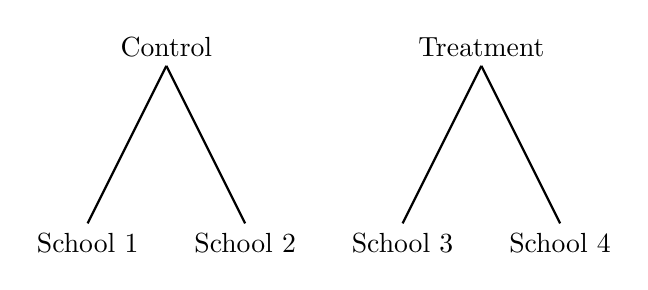
\begin{tikzpicture}
\draw [thick] (3,5) -- (2,3);
\draw [thick] (3,5) -- (4,3);
\draw [thick] (7,5) -- (6,3);
\draw [thick] (7,5) -- (8,3);
\node [above] at (3,5) {Control};
\node [above] at (7,5) {Treatment};

\node [below] at (2,3) {School 1};
\node [below] at (4,3) {School 2};

\node [below] at (6,3) {School 3};
\node [below] at (8,3) {School 4};
\end{tikzpicture}
  \caption{A model}
\end{figure}

We can draw this picture again, replacing the names with the corresponding model notation

\begin{figure}
  \centering
    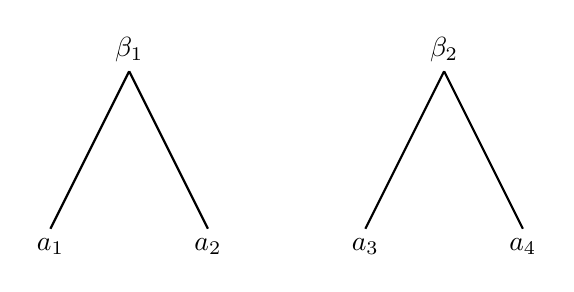
\begin{tikzpicture}
\draw [thick] (3,5) -- (2,3);
\draw [thick] (3,5) -- (4,3);
\draw [thick] (7,5) -- (6,3);
\draw [thick] (7,5) -- (8,3);
\node [above] at (3,5) {$\beta_1$};
\node [above] at (7,5) {$\beta_2$};

\node [below] at (2,3) {$a_1$};
\node [below] at (4,3) {$a_2$};

\node [below] at (6,3) {$a_3$};
\node [below] at (8,3) {$a_4$};
\end{tikzpicture}
   \caption{$y_{ijk} = \mu + a_{jk} + \beta_k + e_{ijk}$}
\end{figure}


As with the random effects model, here we also have two variance components, the between-school and within-school variances, and the total variance net of the fixed treatment effect is the sum of these variance components

\[
a_{jk} \sim N\left(0,\sigma_b^2\right)
\]

\[
e_{ijk} \sim N\left(0,\sigma_w^2\right)
\]

\[
\mbox{var}\left(y_{ijk}|\beta_k\right) = \sigma_T^2  = \sigma_b^2 +\sigma_w^2
\]

Estimating the effects from such a model is possible within the ANOVA framework using a two-way mixed effects model. Suppose we had $p$ treatment groups and $m$ schools per treatment group, each with $n$ students, the test of a treatment effect would be the ratio of the mean squares between treatment groups, which has an expected value that combines all sources of variation

\[
E[MS_{treatment}] = \sigma_w^2+n\sigma_b^2+nm\sum_{k=1}^p\frac{\beta_k^2}{p-1}
\]

this quantity would be divided by the mean squares between schools, but within treatments. Its expected value is the within-school variance component plus the school size times the between school variance component.

\[
E[MS_{schools(treatment)}] = \sigma_w^2+n\sigma_b^2
\]

Thus, the test for treatment effects is expected, again, to be an F-ratio of 1 if the null hypothesis were true

\[
E[F_{null}] = \frac{\sigma_w^2+n\sigma_b^2}{\sigma_w^2+n\sigma_b^2}
\]

and a ratio of greater than 1 if the alternative hypothesis is true

\[
E[F_{alternative}] = \frac{\sigma_w^2+n\sigma_b^2+nm\sum_{k=1}^p\frac{\beta_k^2}{p-1}}{\sigma_w^2+n\sigma_b^2}
\]

As you can see, mixed models are based on the ANOVA framework and have been in use for some time. However, mixed effect regression models, or multilevel models, or hierarchical linear models, allow us to estimate the effects of fixed variables and also the variance components associated with random effects in a regression framework.

We are not limited to just categorical or group factors. For example, we could have a mixed model that suggests that the relationship between an outcome y and an observed linear predictor x is fixed at beta 1, that is, all groups have the same slope for x. However, each group has a random effect that impacts its mean, a, which adjusts the regression intercept value.

\begin{figure}
  \centering
  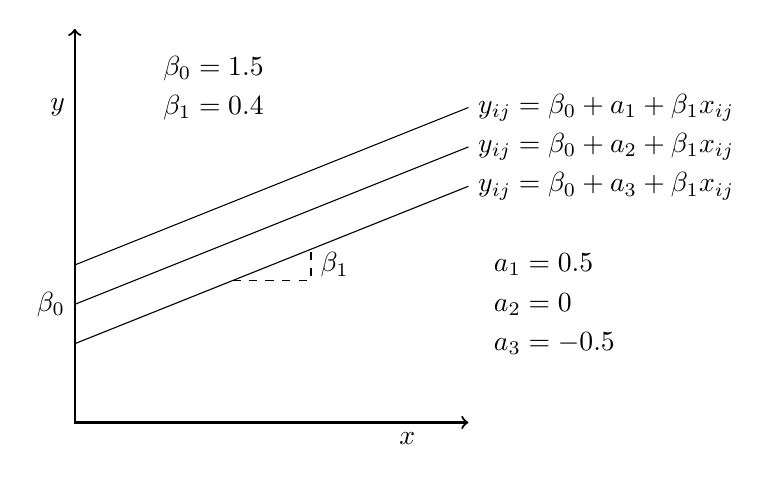
\begin{tikzpicture}
\draw [thick, <->] (0,5) -- (0,0) -- (5,0);
\draw (0,2) -- (5,4);
\draw (0,1.5) -- (5,3.5);
\draw (0,1) -- (5,3);
\node [below right] at (4,0) {$x$};
\node [left] at (0,4) {$y$};
\node [right] at (5,4) {$y_{ij}=\beta_0+a_1+\beta_1x_{ij}$};
\node [right] at (5,3.5) {$y_{ij}=\beta_0+a_2+\beta_1x_{ij}$};
\node [right] at (5,3) {$y_{ij}=\beta_0+a_3+\beta_1x_{ij}$};
\node [left] at (0,1.5) {$\beta_0$};
\draw [dashed, -] (2,1.8) -- (3,1.8) -- (3,2.2);
\node [right] at (3,2) {$\beta_1$};
\node [right] at (5.2,2) {$a_1 = 0.5$};
\node [right] at (5.2,1.5) {$a_2 = 0$};
\node [right] at (5.2,1) {$a_3 = -0.5$};
\node [right] at (1,4.5) {$\beta_0 = 1.5$};
\node [right] at (1,4) {$\beta_1 = 0.4$};
\end{tikzpicture}
  \caption{Model: $y_{ij} = \beta_0+a_j+\beta_1x_{ij}+e_{ij}$}\label{hlmfig}
\end{figure}

In the Figure~\ref{hlmfig} you see three parallel lines, one for each of three hypothetical groups. The model for data that would generate these lines is at the top. It includes two fixed effects, the intercept $\beta_0$ and the slope for $x$, $\beta_1$. We also have a random effect, $a$, that is unique to each group. Since these lines are parallel, they all have the same slope, $\beta_1$, which is equal to about 0.4. Making group 2 the reference group, we see that group one has a positive random effect and that group 3 has a negative random effect. Since group 2 is the reference group, it has no random effect.

\[
y_{ij} = \beta_0+a_j+\beta_1x_{ij}+c_jx_{ij}+e_{ij}
\]

\[
y_{ij} = \beta_0+a_j+\underbrace{\beta_1}_{\text{fixed slope}}x_{ij}+\underbrace{c_j}_{\text{random effect on slope}}x_{ij}+e_{ij}
\]

Of course, the slope of a predictor can also be different for different groups. Thus, slopes can have a random effect as well. We can think of this as another effect for the same predictor variable.

\begin{figure}
  \centering
  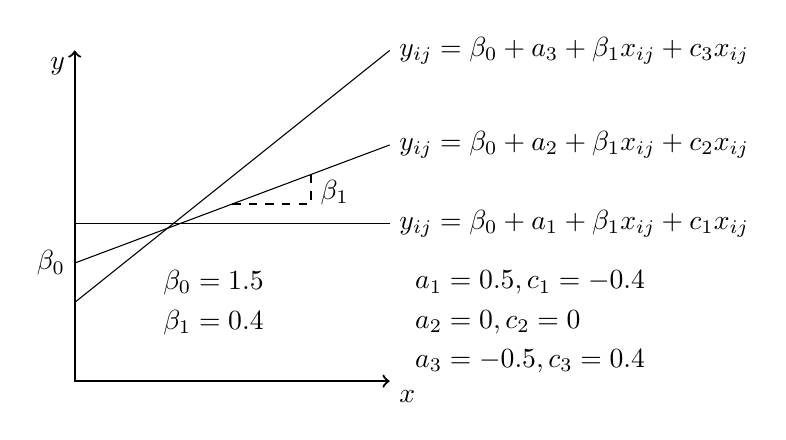
\begin{tikzpicture}
\draw [thick, <->] (0,4.2) -- (0,0) -- (4,0);
\draw (0,2) -- (4,2);
\draw (0,1.5) -- (4,3);
\draw (0,1) -- (4,4.2);
\node [below right] at (4,0) {$x$};
\node [left] at (0,4) {$y$};
\node [right] at (4,2) {$y_{ij}=\beta_0+a_1+\beta_1x_{ij}+c_1x_{ij}$};
\node [right] at (4,3) {$y_{ij}=\beta_0+a_2+\beta_1x_{ij}+c_2x_{ij}$};
\node [right] at (4,4.2) {$y_{ij}=\beta_0+a_3+\beta_1x_{ij}+c_3x_{ij}$};
\node [left] at (0,1.5) {$\beta_0$};
\draw [dashed, -] (2,2.25) -- (3,2.25) -- (3,2.7);
\node [right] at (3,2.4) {$\beta_1$};
\node [right] at (4.2,1.25) {$a_1 = 0.5, c_1 = -0.4$};
\node [right] at (4.2,.75) {$a_2 = 0, c_2 = 0$};
\node [right] at (4.2,.25) {$a_3 = -0.5, c_3 = 0.4$};
\node [right] at (1,1.25) {$\beta_0 = 1.5$};
\node [right] at (1,.75) {$\beta_1 = 0.4$};
\end{tikzpicture}
  \caption{Model: $y_{ij} = \beta_0+a_j+\beta_1x_{ij}+c_jx_{ij}+e_{ij}$}\label{hlmfig2}
\end{figure}


Again, in Figure~\ref{hlmfig2} you see three lines, but now they are no longer parallel, one for each of three hypothetical groups. The model for data that would generate these lines is at the top. It includes two fixed effects, the intercept $\beta_0$ and the slope for x, $\beta_1$. We now also have two random effects, $a$ and $c$, that are unique to each group. These lines all have the unique intercepts and slopes. The average slope is for group 2, $\beta_0$, and the average slope is also for group 2, $\beta_1$. The random effects for group 2 are also 0. Making group 2 the reference group, we see that group one has a positive random effect on the intercept, but a negative random effect for the slope and that group 3 has a negative random effect for the intercept, but a positive random effect for the slope.

While many things are estimated from multilevel models, multilevel analyses share the goals of many statistical applications in that the most important elements that come from the statistical output are means and variances. In our case, we specifically estimate fixed effects, which are estimates of means, and the variances of random effects. Recall the mixed effects model we considered at the end of the previous video, where we had a fixed intercept, a random effect on the intercept, a fixed slope, a random effect on the slope, and a residual.\footnote{Remember, the rule in this video series is that fixed effects are represented by Greek letters and random effects are represented by Roman letters. if you need a mnemonic device, perhaps you can remember that F (for fixed) comes before G (for Greek), and that R is for Roman, and also for Random.}

\[
y_{ij} = \beta_0+a_j+\beta_1x_{ij}+c_jx_{ij}+e_{ij}
\]

So, looking at the equation again, we see that the intercept, beta 0 is a fixed effect, which is a mean, a is the random effect of the group on the mean, for which we can estimate the variance, beta 1 is the slope, which is a difference in the mean due to a change in x, which is fixed, and c is the random difference in this slope by group, for which we estimate the variance. We also estimate the variance of the residuals.

So, whenever a quantity is a fixed effect, multilevel models will estimate a mean or difference in means of some sort, and whenever something is a random effect, multilevel models provide a variance. This is somewhat of a simplification, because most software packages can actually predict a random effect for a group.

Technical details of the computations that deliver the output are beyond the scope of these notes. However, it is worth-while to mention that most of the time, these models are estimated by maximum likelihood algorithms. It is possible to estimate these models using other means, but most mainstream applications are done within the frequentist maximum likelihood paradigm. There is, however, one important distinction within maximum likelihood.

Some software will use what we call full maximum likelihood, which will estimate all parameters in the same way regardless of sample size or number of parameters. This method is preferable for using likelihood ratio tests to test nested models, for example. Another method is called Restricted maximum likelihood, which takes into account the sample size and degrees of freedom in the estimation of the random effects.  The fixed effects are not different, but the random effects are generally larger. This will then give the same answers as an analysis using ANVOA formulas. However, likelihood ratio tests are not possible. With large samples, the difference is likely to be negligible, but it is important to keep an eye on what the software is doing.

\section{Assumptions}

Before we continue, it is important that we discuss some assumptions for the models we are about to employ. The reason why complicated problems can be defensibly reduced to relatively few formulas is because the statisticians that worked on these formulas made assumptions. If these assumptions are not met, we probably should find a more complicated tool. So, this is important.

I won't list all the assumptions here, because many of the assumptions of a mixed linear model are those of a fixed linear model, such as the outcome is a linear function of the predictors, the expected value of any random effect is zero, the values of the predictors are not random (although their effects may be), the predictors are not perfectly correlated, and so on.

The assumptions we need to bear in mind are about the random effects, and generally they are similar to the assumptions of the one-level linear model residuals.


\begin{itemize}
  \item Assumption: the within-group residuals are normally distributed, independent (within group) and have a constant variance (across groups)
  \item Assumption: the within-group residuals are not correlated with the random effects
  \item Assumption: the between-group residuals are independent and come from a multivariate normal distribution
\end{itemize}

Regarding the within group residuals, we assume they are independent within the group. That is, for example, that students were independently sampled within the school, or neighborhood, etc. We also assume that the residuals from the model are normally distributed (for the linear mixed model) and have a constant variance that is common across groups. This is akin to the equal variances between groups that is assumed in one-way ANOVA or a t-test. If time is nested within person, this could be a problem, as time is usually serially correlated. However, this can be solved with a more complex model.

The within group residuals need to be independent of the group-level random effects. That is, if a group has a higher mean, that can't be related to the average value of the within-group residuals. This is a key assumption to any random-effect model, and it is difficult to test. In econometrics, often they will fit a random-effect model with generalized least squares and compare that to a purely fixed effects model with what's called a Hausman text.

Finally, the between group random effects, differences in means or slopes, are assumed to be independent and come from a multivariate normal distribution. That is, each group is assumed to be independently sampled, so their random effects are independent. Technically, this means that if you are working with census tracts that are next to each other, you need to account for the spacial dependence somehow. This also precludes the use of time as a grouping variable, say, year, for instance, because there is surely going to be serial autocorrelation across years.

\section{Notation}

Our discussion in these notes will offer a two notation schemes for writing down a multilevel model: the HLM notation and the mixed model notation, both of which are useful for organizing your thoughts about that you are modeling. We then move to understand what actually is estimated and output from the computer and how to interpret those values.

One notation for writing down a multilevel model was popularized by Raudenbush and Bryk in their work on Hierarchical Linear Models, or HLM. This notation splits up the fixed and random effects into into different levels of the data.  For example, if students are nested in schools, then we have two levels--students and schools--and we then write down a level 1 model and various level 2 models.

\subsection{Unconditional ANOVA model in HLM notation}

Let's start with a simple ANOVA model, which is a model without covariates that only estimates the variance components of random effects. This is also sometimes called an unconditional model.

Unconditional ANOVA model in HLM notation

\[
y_{ij} = \beta_{0j}+e_{ij}
\]
\[
\beta_{0j} = \gamma_{00}+u_{0j}
\]

We see two equations. The first is the level-1 model, that says that the outcome y for unit i in group j is a function of a group-specific mean, beta 0 j, and a deviation from that group specific mean which is the level 1 residual term. Next, the following equation is the level 2 equation, which specifies that the group averages are a function of an average of the group averages, gamma 0 0, plus a deviation of the group's specific average from this average of averages.

\[
\underbrace{y_{ij} = \beta_{0j}+e_{ij}}_{\text{Level 1 model}}
\]
\[
\underbrace{\beta_{0j} = \gamma_{00}+u_{0j}}_{\text{Level 2 model}}
\]

\[
y_{ij} = \beta_{0j}+\underbrace{e_{ij}}_{\text{Random}}
\]
\[
\beta_{0j} = \underbrace{\gamma_{00}}_{\text{Fixed}}+\underbrace{u_{0j}}_{\text{Random}}
\]

You may be wondering why I didn't call out the betas. The reason is that beta 0 j is just a place holder. Now, we move to mixed notation that replaces beta 0 j in the level 1 model with the results of the level 2 model

\[
y_{ij} = \beta_{0j}+e_{ij}
\]
\[
\beta_{0j} = \gamma_{00}+u_{0j}
\]
Replace $\beta$'s for mixed notation

\[
y_{ij} = \underbrace{\gamma_{00}+u_{0j}}_{\beta_{0j}}+e_{ij}
\]

Unconditional ANOVA model in mixed notation

\[
y_{ij} = \gamma_{00}+u_{0j}+e_{ij}
\]

Now, each element of the equation is either fixed or random

\[
y_{ij} = \underbrace{\gamma_{00}}_{\text{Fixed}}+\underbrace{u_{0j}+e_{ij}}_{\text{Random}}
\]

This equation takes the same form as the one-way random effects ANOVA model, earlier. The grand mean is estimated with the fixed effect $\mu$ in the ANOVA notation, and $\gamma_{00}$ in the mixed notation. The deviation of each group's mean from the grand mean is $a_j$ in ANOVA notation, and $u_{0j}$ in the mixed notation, and the within-group residual is the same, $e_{ij}$.

One-way random effects ANOVA model

\[
y_{ij} = \mu + a_j+e_{ij}
\]

Unconditional ANOVA model in mixed notation

\[
y_{ij} = \gamma_{00}+u_{0j}+e_{ij}
\]
$\mbox{Grand mean} = \mu = \gamma_{00}$

$\mbox{Random group effect} = a_j = u_{0j} $

$\mbox{Within-group residual} = e_{ij}$

And like the oneway random effects model, we have two components of variance, the group mean deviations from the grand mean are distributed normally with a mean of 0 and a variance of $\sigma^2_b$, and the within-group residuals are distributed normally with a mean of 0 and a variance of $\sigma^2_w$. The total variation is then the sum of the two variance components.

Variance components from mixed model

\[
y_{ij} = \gamma_{00}+u_{0j}+e_{ij}
\]

\[
u_{0j} \sim N\left(0, \sigma_b^2\right)
\]

\[
e_{ij} \sim N\left(0, \sigma_w^2\right)
\]

\[
\sigma_T^2 = \sigma_b^2+\sigma_w^2
\]

\section{Two-level models}

\subsection{Random intercepts}

Now, let's write down a model with a single level 1 predictor.  For now, let's assume that the effect of this predictor is fixed, or it is the same for all groups.

Using the HLM notation, we can write down the level 1 and level 2 models as we did before. We add a predictor, x, to the level one model. This means we also add a slope, $\beta_{1j}$ to the level one model. We then need to add another level 2 equation, where $\beta_{1j}$ is now a function of $\gamma_{10}$, but since we are fixing this effect, there is no random element to it.

Model with level 1 covariate with fixed slope in HLM notation

\[
y_{ij} = \beta_{0j}+\beta_{1j}x_{ij}+e_{ij}
\]
\[
\beta_{0j} = \gamma_{00}+u_{0j}
\]
\[
\beta_{1j} = \gamma_{10}
\]

\[
\underbrace{y_{ij} = \beta_{0j}+\beta_{1j}x_{ij}+e_{ij}}_{\text{Level 1}}
\]
\[
\mbox{Level 2}
\begin{cases}
    \beta_{0j} = \gamma_{00}+u_{0j}  \\
    \beta_{1j} = \gamma_{10}
\end{cases}
\]

Of course, we can replace the beta's with their formulas to form the mixed-notation equation

\[
y_{ij} = \beta_{0j}+\beta_{1j}x_{ij}+e_{ij}
\]
\[
\beta_{0j} = \gamma_{00}+u_{0j}
\]
\[
\beta_{1j} = \gamma_{10}
\]
Replace $\beta$'s

\[
y_{ij} = \underbrace{\gamma_{00}+u_{0j}}_{\beta_{0j}}+\underbrace{\gamma_{10}}_{\beta_{1j}}x_{ij}+e_{ij}
\]

Which leaves us with the mixed notation, with a little rearranging, moving all the random elements to the end of the formula.

\[
y_{ij} = \gamma_{00}+\gamma_{10}x_{ij}+u_{0j}+e_{ij}
\]

\[
y_{ij} = \underbrace{\gamma_{00}+\gamma_{10}x_{ij}}_{\text{Fixed}}+\underbrace{u_{0j}+e_{ij}}_{\text{Random}}
\]

\subsection{Random slopes}

Next, we can relax the constraint that the effect of $x$ is the same for all schools. This adds another random effect, $u_{1j}$ to the group-specific slope for $x$.

Model with level 1 covariate with a random slope in HLM notation

\[
y_{ij} = \beta_{0j}+\beta_{1j}x_{ij}+e_{ij}
\]
\[
\beta_{0j} = \gamma_{00}+u_{0j}
\]
\[
\beta_{1j} = \gamma_{10}+u_{1j}
\]

Let's consider the meaning of $\gamma_{10}$ and $u_{1j}$. If $\beta_{1j}$ is the slope for our level 1 predictor specific to each group, then $\gamma_{10}$ is an average of those slopes, and $u_{1j}$ is how each group deviates from that average slope. Thus, this model will estimate a third variance component.
\[
\underbrace{y_{ij} = \beta_{0j}+\beta_{1j}x_{ij}+e_{ij}}_{\text{Level 1}}
\]
\[
\mbox{Level 2}
\begin{cases}
    \beta_{0j} = \gamma_{00}+u_{0j}  \\
    \beta_{1j} = \gamma_{10}+u_{1j}
\end{cases}
\]

Now, since we have multiple variance components, we need to think of them as distributed in a multivariate normal distribution. That is, since each group has a couple random effects, it makes sense to consider how they co-vary. Thus, not only do we have a variance for each random effect, we also have the covariances between each random effect at level 2. There are many ways to write this down, for simplicity let's put all the variances and covariances at level 2 into a matrix called $U$

Variance and covariance components from model with level 1 covariate with a random slope
Level 2

\[
\mbox{\textbf{U}} =
\begin{bmatrix}
	\mbox{var}\left(u_{0j}\right) & \mbox{cov}\left(u_{0j},u_{1j}\right) \\
	\mbox{cov}\left(u_{1j},u_{0j}\right) & \mbox{var}\left(u_{1j}\right)
\end{bmatrix}
\]

Level 1

\[
e_{ij} \sim N\left(0, \sigma_w^2\right)
\]

Another consequence of this model is that a neat and tidy concept of an intraclass correlation is lost, since its a little difficult to define a total variance with random slopes.

Moving to mixed notation, we can of course, replace the beta's with their formulas to form the mixed-notation equation

\[
y_{ij} = \beta_{0j}+\beta_{1j}x_{ij}+e_{ij}
\]
\[
\beta_{0j} = \gamma_{00}+u_{0j}
\]
\[
\beta_{1j} = \gamma_{10}+u_{1j}
\]
Replace $\beta$'s

\[
y_{ij} = \underbrace{\gamma_{00}+u_{0j}}_{\beta_{0j}}+\underbrace{\left(\gamma_{10}+u_{1j}\right)}_{\beta_{1j}}x_{ij}+e_{ij}
\]

Which leaves us with the mixed notation, with a little rearranging, distributing $x_{ij}$ across to both $\gamma_{10}$ and $u_{1j}$, and moving all the random elements to the end of the formula.

Model with level 1 covariate with a random slope in mixed notation

\[
y_{ij} = \gamma_{00}+\gamma_{10}x_{ij}+u_{0j}+u_{1j}x_{ij}+e_{ij}
\]

Now, we see that the predictor $x$ is interacting with a random effect. This is sometimes called a heteroskedastic error term, since now an error term has non-constant variance because it relates to the value of one of the predictors. Many econometric techniques for solving heteroskedasticity involve modeling the relationship between error and predictors, and here we see we do it directly (at least in a linear fashion)

\[
y_{ij} = \underbrace{\gamma_{00}+\gamma_{10}x_{ij}}_{\text{Fixed}}+\underbrace{u_{0j}+u_{1j}x_{ij}+e_{ij}}_{\text{Random}}
\]


As many know, a correlation is a standardized covariance. The way to standardize a covariance is to divide it by the square-root of the product of the two variables' variances. This allows us to posit a correlation between the random effects.

\[
\mbox{corr}\left(u_{0j},u_{1j}\right) = \frac{\mbox{cov}\left(u_{0j},u_{1j}\right)}{\sqrt{\mbox{var}\left(u_{0j}\right)\mbox{var}\left(u_{1j}\right)}}
\]



\subsubsection{Model with level 2 covariate}

Next, let us consider a model without a level 1 predictor, but instead a level 2 predictor, which we will call $w_j$. In the HLM notation, we have our level 1 model which looks much like the ANOVA model, but now we have a variable entered at level 2

Model with level 2 covariate in HLM notation

\[
y_{ij} = \beta_{0j}+e_{ij}
\]
\[
\beta_{0j} = \gamma_{00}+\gamma_{01}w_j+u_{0j}
\]

\[
\underbrace{y_{ij} = \beta_{0j}+e_{ij}}_{\text{Level 1}}
\]
\[
\underbrace{\beta_{0j} = \gamma_{00}+\gamma_{01}w_j+u_{0j}}_{\text{Level 2}}
\]

Of course, we can replace the beta with the level 2 formula to form the mixed-notation equation Which leaves us with the mixed notation, with a little rearranging, moving all the random elements to the end of the formula.\footnote{It's worth mentioning that this is equivalent model as the hierarchical two-way mixed model we discussed before, where the covariate is a characteristic of the group. In a cluster randomized trial, this covariate is the treatment indicator.}

Model with level 2 covariate in mixed notation

\[
y_{ij} = \gamma_{00}+\gamma_{01}w_j+u_{0j}+e_{ij}
\]

\subsubsection{Model with level 1 covariate with a fixed slope and a level 2 covariate}

Next, let us consider a model with a level 1 predictor with a fixed slope and a level 2 covariates. In the HLM notation, we have our level 1 model which includes the covariate and its slope (but no random effect), and now we have a variable entered at level 2

Model with level 1 covariate with a fixed slope and a level 2 covariate in HLM notation

\[
y_{ij} = \beta_{0j}+\beta_{1j}x_{ij}+e_{ij}
\]
\[
\beta_{0j} = \gamma_{00}+\gamma_{01}w_j+u_{0j}
\]
\[
\beta_{0j} = \gamma_{10}
\]

\[
\underbrace{y_{ij} = \beta_{0j}+\beta_{1j}x_{ij}+e_{ij}}_{\text{Level 1}}
\]
\[
\mbox{Level 2}
\begin{cases}
    \beta_{0j} = \gamma_{00}+\gamma_{01}w_j+u_{0j}  \\
    \beta_{1j} = \gamma_{10}
\end{cases}
\]

Like before, we can replace the betas with the level 2 formulas to form the mixed-notation equation, With a little rearranging, moving all the random elements to the end of the formula.

Model with level 1 covariate with a fixed slope and a level 2 covariate in mixed notation

\[
y_{ij} = \gamma_{00}+\gamma_{01}w_j+\gamma_{10}x_{ij}+u_{0j}+e_{ij}
\]

\subsubsection{Model with level 1 covariate with a fixed slope, a 2 covariate, and an interaction between the level 1 and level 2 covariate}

Next, let us consider a model with a level 1 predictor with a fixed slope, a level 2 covariate, and now an interaction between the level 1 and level 2 covariates. In the HLM notation, we think of the level 1 slope, beta 1 j as an outcome regressed on the level 2 covariate

Model with level 1 covariate with a fixed slope, a 2 covariate, and an interaction between the level 1 and level 2 covariate in HLM notation

\[
y_{ij} = \beta_{0j}+\beta_{1j}x_{ij}+e_{ij}
\]
\[
\beta_{0j} = \gamma_{00}+\gamma_{01}w_j+u_{0j}
\]
\[
\beta_{0j} = \gamma_{10}+\gamma_{11}w_j
\]

Here, $\gamma_{11}$ is often called a cross level effect, because it proposes that a level 2 characteristic influences the slope of a level 1 characteristic. Often, people think that this is something only HLM can do. However, when we convert this to the mixed model notation we will see that this is simply an interaction.

Model with level 1 covariate with a fixed slope, a 2 covariate, and an interaction between the level 1 and level 2 covariate in HLM notation

\[
\underbrace{y_{ij} = \beta_{0j}+\beta_{1j}x_{ij}+e_{ij}}_{\text{Level 1}}
\]
\[
\mbox{Level 2}
\begin{cases}
    \beta_{0j} = \gamma_{00}+\gamma_{01}w_j+u_{0j}  \\
    \beta_{1j} = \gamma_{10}+\gamma_{11}w_j
\end{cases}
\]

Like before, we can replace the betas with the level 2 formulas to form the mixed-notation equation, With a little rearranging, moving all the random elements to the end of the formula.

Model with level 1 covariate with a fixed slope, a 2 covariate, and an interaction between the level 1 and level 2 covariate \\

HLM notation

\[
y_{ij} = \beta_{0j}+\beta_{1j}x_{ij}+e_{ij}
\]
\[
\beta_{0j} = \gamma_{00}+\gamma_{01}w_j+u_{0j}
\]
\[
\beta_{0j} = \gamma_{10}+\gamma_{11}w_j
\]

Replace

\[
y_{ij} = \underbrace{\gamma_{00}+\gamma_{01}w_j+u_{0j}}_{\beta_{0j}}+\underbrace{\left(\gamma_{10}+\gamma_{11}w_j\right)}_{\beta_{1j}}x_{ij}+e_{ij}
\]

Rearrange for mixed notation

\[
y_{ij} = \gamma_{00} + \gamma_{01}w_j + \gamma_{10}x_{ij}+\gamma_{11}w_jx_{ij}+u_{0j}+e_{ij}
\]

Here, we see that $\gamma_{11}$ is just the slope for the interaction between the level 1 covariate, $x$, and the level 2 covariate, $w$.

\subsubsection{Model with level 1 covariate with a random slope and a level 2 covariate}

Next, let us consider a model with a level 1 predictor with a random slope and a level 2 covariate. In the HLM notation, we have our level 1 model which includes the covariate and its slope, and now we have a variable entered at level 2

Model with level 1 covariate with a random slope and a level 2 covariate in HLM notation

\[
y_{ij} = \beta_{0j}+\beta_{1j}x_{ij}+e_{ij}
\]
\[
\beta_{0j} = \gamma_{00}+\gamma_{01}w_j+u_{0j}
\]
\[
\beta_{0j} = \gamma_{10}+u_{1j}
\]

\[
\underbrace{y_{ij} = \beta_{0j}+\beta_{1j}x_{ij}+e_{ij}}_{\text{Level 1}}
\]
\[
\mbox{Level 2}
\begin{cases}
    \beta_{0j} = \gamma_{00}+\gamma_{01}w_j+u_{0j}  \\
    \beta_{1j} = \gamma_{10}+u_{1j}
\end{cases}
\]


Like before, we can replace the betas with the level 2 formulas to form the mixed-notation equation, With a little rearranging, moving all the random elements to the end of the formula.

Model with level 1 covariate with a random slope and a level 2 covariate in mixed notation

\[
y_{ij} = \gamma_{00}+\gamma_{01}w_j+\gamma_{10}x_{ij}+u_{0j}+x_{ij}u_{1j}+e_{ij}
\]

\subsubsection{Model with level 1 covariate with a random slope, a level 2 covariate, and an interaction between the level 1 and level 2 covariate}

This will be the most complicated model we consider in these notes. Let us consider a model with a level 1 predictor with a random slope, a level 2 covariate, and an interaction between the level 1 and level 2 covariates. In the HLM notation, we think of the level 1 slope, $\beta_{1j}$ as an outcome regressed on the level 2 covariate with a random effect

Model with level 1 covariate with a random slope, a 2 covariate, and an interaction between the level 1 and level 2 covariate in HLM notation

\[
y_{ij} = \beta_{0j}+\beta_{1j}x_{ij}+e_{ij}
\]
\[
\beta_{0j} = \gamma_{00}+\gamma_{01}w_j+u_{0j}
\]
\[
\beta_{0j} = \gamma_{10}+\gamma_{11}w_j+u_{1j}
\]

Here, $\gamma_{11}$ is still a cross level effect, because it proposes that a level 2 characteristics influences the slope of a level 1 characteristic. However, when we convert this to the mixed model notation we will see that this is still simply an interaction.

Model with level 1 covariate with a random slope, a level 2 covariate, and an interaction between the level 1 and level 2 covariate in HLM notation

\[
\underbrace{y_{ij} = \beta_{0j}+\beta_{1j}x_{ij}+e_{ij}}_{\text{Level 1}}
\]
\[
\mbox{Level 2}
\begin{cases}
    \beta_{0j} = \gamma_{00}+\gamma_{01}w_j+u_{0j}  \\
    \beta_{1j} = \gamma_{10}+\gamma_{11}w_j+u_{1j}
\end{cases}
\]

Like before, we can replace the betas with the level 2 formulas to form the mixed-notation equation, With a little rearranging, moving all the random elements to the end of the formula.

HLM notation

\[
y_{ij} = \beta_{0j}+\beta_{1j}x_{ij}+e_{ij}
\]
\[
\beta_{0j} = \gamma_{00}+\gamma_{01}w_j+u_{0j}
\]
\[
\beta_{0j} = \gamma_{10}+\gamma_{11}w_j+u_{1j}
\]

Replace

\[
y_{ij} = \underbrace{\gamma_{00}+\gamma_{01}w_j+u_{0j}}_{\beta_{0j}}+\underbrace{\left(\gamma_{10}+\gamma_{11}w_j+u_{1j}\right)}_{\beta_{1j}}x_{ij}+e_{ij}
\]

Rearrange for mixed notation

\[
y_{ij} = \gamma_{00} + \gamma_{01}w_j + \gamma_{10}x_{ij}+\gamma_{11}w_jx_{ij}+u_{0j}+x_{ij}u_{1j}+e_{ij}
\]

Here, we see that again $\gamma_{11}$ is just the slope for the interaction between the level 1 covariate, $x$, and the level 2 covariate, $w$.

\subsection{Evaluating the model}

As with any statistical technique, inference asks two basic questions. First, how well does the model fit the data? Second, what is the precision of the parameters, which is the fundamental question for evaluating hypothesis tests.

\begin{itemize}
	\item How well does the model fit the data?
	\item What is the precision of the parameters (hypothesis testing)?
\end{itemize}

While there are many different ways to assess fit to the data, in this video we will simply focus on two tests: differences in deviance based on the log likelihood and proportional reduction in variance components

\subsubsection{Likelihood}

If you estimate a linear multilevel model with full maximum likelihood, it is possible to compare two models that differ on a nested set of parameters (which can be fixed effects or variances of random effects) using a $\chi$-square test.

\[
D = -2\times \mbox{ln}\left(L\right)
\]

This is accomplished by calculating the deviance of the two models to compare, then finding the difference. Deviance, or D, is negative 2 times the log likelihood of the model that is maximized during the estimation procedure.

Model 0:

\[
y_{ij}= \gamma_{00} + \gamma_{10}x_{ij} + u_{0j} + e_{ij}
\]

Model 1:

\[
y_{ij}= \gamma_{00} + \gamma_{10}x_{ij} + u_{0j} +x_{ij}u_{1j} + e_{ij}
\]

For example, suppose we had a choice between two models, a model with a level 1 covariate with a fixed slope, and a model with the same level 1 covariate with a random slope. We want to see if allowing the level 1 covariate's slope to have a random effect really fit the data better.  The way we can test the statistical significance of the random effect by calculating the deviance for each model, then finding the difference between the two, which has a $\chi$-square distribution with $p$ degrees of freedom, where $p$ is the number of new parameters.

\[
\mbox{Test} = D_0 - D_1
\]
\[
\mbox{Test} \sim \chi^2_p
\]
$p$ is the number of new parameters


With this test in hand, we simply look up the critical chi-square value associated with the number of new parameters. For our example, we have 1 new random effect, so our critical value is 3.842.

Another way to test the usefulness of adding variables with fixed slopes or level 2 variables is to examine how the variance components change proportionally. Again, suppose two models, the first a unconditional ANOVA model, and a second model with a level 2 covariate.

Fixed Effects: Wald tests

Different software does this in different ways, HLM will give chi-square tests for VCs

If you use full ML, you can do LR tests for random effects

\section{Example analysis}

As an example to apply everything we have learned, we will analyze the Early Childhood Longitudinal Study 1998 Kindergarten Cohort. This data set contains about eighteen thousand students across about a thirteen hundred schools.   We will examine their Spring Math scores. To give you a sense of the distribution, on your screen his a histogram of the scores in 10 point buckets. The mean score is about 36, with a standard deviation of approximately 12 points.

\begin{figure}
  \centering
  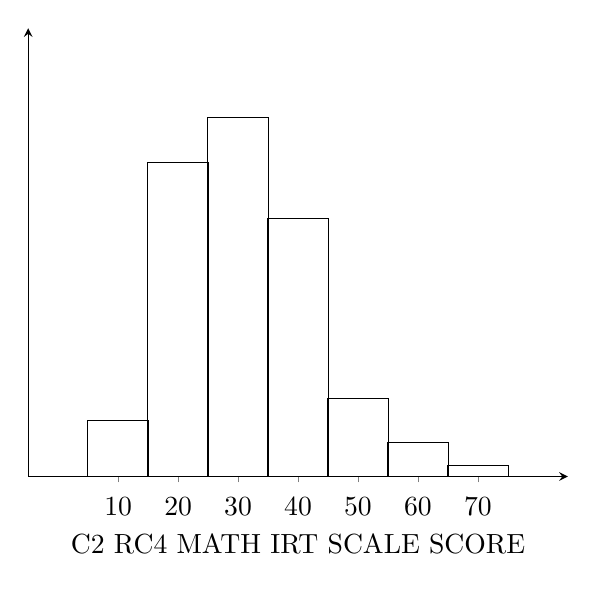
\begin{tikzpicture}
    \begin{axis}[
      ybar,
      bar width=22pt,
      xlabel={C2 RC4 MATH IRT SCALE SCORE},
      ymin=0,
      ymax = 40,
      ytick=\empty,
      xtick=data,
      axis x line=bottom,
      axis y line=left,
      enlarge x limits=.25,
      xticklabel style={anchor=base,yshift=-\baselineskip},
    ]
      \addplot[fill=white] coordinates {
        (10,5)
        (20,28)
        (30,32)
        (40,23)
        (50,7)
        (60,3)
        (70,1)
      };
    \end{axis}
  \end{tikzpicture}
  \caption{Distribution of Spring Kindergarten Math Scores ($\bar{y} = 36, s = 12$)}\label{eclsdist}
\end{figure}

The key predictor we will be using is parents highest level of education. Originally recorded as a ordinal variable, I have taken the liberty of recoding it as a continuous years of education variable. Its mean is about 14 years with a standard deviation of about 2.5 years of schooling.

\begin{figure}
  \centering
  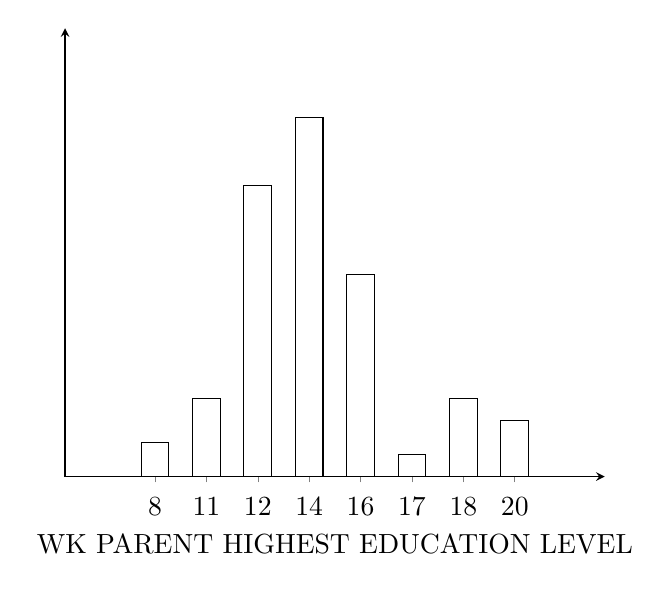
\begin{tikzpicture}
    \begin{axis}[
      ybar,
      bar width=10pt,
      xlabel={WK PARENT HIGHEST EDUCATION LEVEL},
      ymin=0,
      ymax = 40,
      ytick=\empty,
      xtick=data,
      axis x line=bottom,
      axis y line=left,
      enlarge x limits=.25,
      symbolic x coords={8,11,12,14,16,17,18,20},
      xticklabel style={anchor=base,yshift=-\baselineskip},
    ]
      \addplot[fill=white] coordinates {
        (8,3)
        (11,7)
        (12,26)
        (14,32)
        (16,18)
        (17,2)
        (18,7)
        (20,5)
      };
    \end{axis}
  \end{tikzpicture}
  \caption{Distribution of Parent Years of Education ($\bar{x} = 14, s = 2.5$)}\label{}
\end{figure}

Finally, about a quarter of the students in the sample attend a private school, and that will be our school level variable.

\subsection{Unconditional ANOVA model}

What does such an analysis look like? If we use the ECLS-K data where students are nested in schools, we can fit the ANOVA model. The results appear on the screen. The table on the screen is organized with the fixed effects on top, and the variances of the random effects on the bottom.  Looking at gamma 00, the fixed intercept, we see that the average school-average is about 36 points. Next, looking at the random effects, we see that the variance of the between-group differences is about 33, and the within-group residual has a variance of about 112.

\begin{table}
  \centering
  \begin{center}

\begin{tabular}{llrr}
\hline
\multicolumn{4}{l}{Fixed} 			 \\
\hline
$\gamma_{00}$	&	Intercept    	&   36.142 &   (0.190)  \\
\hline
\multicolumn{4}{l}{Random}	  \\
\hline
	
$\mbox{var}\left(u_{0j}\right)$	&	Intercept    	&   33.011  \\
$\mbox{var}\left(e_{ij}\right)$ 		&	Residual	& 	 112.319   \\
\hline
Log-likelihood 			& -71299.223 \\
\hline
\multicolumn{4}{l}{SEs of fixed effects in parentheses} \\
\multicolumn{4}{l}{Source: ECLS-K 1998} \\
\hline
\end{tabular}
\end{center}
  \caption{Estimates for unconditional ANOVA model}\label{ecls1}
\end{table}

From these results, we can also calculate an intraclass correlation. Using the results from the ANOVA analysis, we see that 23 percent of the variation occurs at the school level, or that the correlation among student in the same school is about 0.23.

\[
ICC = \frac{\mbox{var}\left(u_{0j}\right)}{\mbox{var}\left(u_{0j}\right)+\mbox{var}\left(e_{ij}\right)}
\]
\[
ICC = \frac{\sigma_b^2}{\sigma_b^2+\sigma_w^2}
\]
\[
ICC = \frac{33.011}{33.011+112.319} = 0.227
\]

\subsection{Model with level 1 covariate with fixed slope}

Now, let's return to our example analysis. Here, x is parental education, in years, for the child. One other wrinkle to this is that we always want to be sure to control the meaning of the intercept.  To that end, let's center parental education on 12 years. If parents' education is less than 12 years, it will be a negative value, if it is 12 years, it will be 0, and greater than 12 years will be a positive value. We will discuss centering in greater detail later. For now, just realize that the intercept is the average of the school mean of a child's score when parents have a high school education.

\begin{table}
  \centering
  \begin{center}
	\begin{tabular}{llrr}
\hline
\multicolumn{4}{l}{Fixed} 			 \\
\hline
$\gamma_{00}$	&	Intercept    	&   15.407 &   (0.521)   \\
$\gamma_{10}$    &	Parent Education    	& 1.483 &   (0.036)    \\
\hline
\multicolumn{4}{l}{Random}	  \\
\hline
	
$\mbox{var}\left(u_{0j}\right)$	&	Intercept    	&   17.543  \\

$\mbox{var}\left(e_{ij}\right)$  		&	Residual	& 	106.076  \\
\hline
Log-likelihood 	&		 -70521.614 \\
\hline
\multicolumn{4}{l}{SEs of fixed effects in parentheses} \\
\multicolumn{4}{l}{Source: ECLS-K 1998} \\
\hline
\end{tabular}
\end{center}
  \caption{Estimates for model with level 1 covariate with fixed slope}\label{ecls2}
\end{table}

OK, here are the results. First, let's look at the fixed intercept effect. If a child's parents have a high school education, because we centered our predictor on 12 years, the average of the school averages for children is a score of about 33. Next, looking at the fixed effect for parental education, we see that for each year greater than high school, this value increases by almost a point and a half. Given these effects, the variance of the level 2 deviations from the intercept is now about 17 and a half, and the variance of the within-group residuals is about 106. It is worth noting that adding this one covariate has reduced the random variance at each level.

\section*{For more information}
For comprehensive treatment of mixed and hierarchical linear models, see \citep{hlm}. For discussions of variance components and centering strategies in multilevel modeling, consult \citep{fox}. Additional perspectives on causal inference in clustered data contexts can be found in \citep{kenny1975quasi} and \citep{cameron2005microeconometrics}.

\subsection{Centering}
\subsubsection{Grand mean centering}
\subsubsection{Group mean centering}


\section{Three-level models}
\subsection{Random intercepts}
\subsection{Random slopes}
\subsection{Cross-level interactions}

\section{Cross-classified models}
\subsection{Random intercepts}


